% Copyright (c) 2026 Barry Malachy, Tegan Massey, Simon Rudkin, Frances Stratton-Killick, Martha Surman. Manuscript text not MIT-licensed.
\documentclass[11pt,a4paper]{article}
\usepackage[margin=2.5cm]{geometry}
\usepackage{graphicx}
\usepackage{booktabs}
\usepackage{threeparttable}
\usepackage{amsmath}
\usepackage{microtype}
\usepackage{setspace}
\usepackage{caption}
\usepackage{subcaption}
\usepackage{placeins}
\usepackage[hidelinks]{hyperref}
\usepackage{natbib}
\usepackage{lineno}
\onehalfspacing
\linenumbers

\title{Similar Food-Access Scores, Different Barriers: Capturing Food-Access Profiles in England}
\author{Barry Malachy, Tegan Massey, Simon Rudkin\thanks{Corresponding author: Simon Rudkin, Department of Social Statistics, University of Manchester, Oxford Road, Manchester M13 9PL, United Kingdom. Email: \texttt{simon.rudkin@manchester.ac.uk}.}, Frances Stratton-Killick, Martha Surman\\Department of Social Statistics, University of Manchester}
\date{}

\begin{document}
\maketitle

\begin{abstract}
Food-access measures often combine retail proximity, household car availability and income deprivation into a single indicator. Such scores can identify areas facing greater constraint, but they can hide why access is constrained. Using all 33,755 English Lower-layer Super Output Areas, we examine retail proximity, household car availability and income deprivation jointly rather than reducing them immediately to one measure. Distinct local food-access profiles can have almost identical overall levels of constraint while reflecting sharply different combinations of barriers, and the finding persists across alternative analytical specifications. Similar barrier profiles also recur across geographically distant places, while contrasting profiles can occur close together. Our results distinguish the overall level of food-access constraint from the barriers underlying it. Composite scores can therefore support place-based prioritisation, but barrier composition should remain visible when interpreting what a similar score means and deciding which aspects of local food access require further assessment.
\end{abstract}

\noindent\textbf{Keywords:} food access; food deserts; Ball Mapper; topological data analysis; household car availability; income deprivation

\section{Introduction}
Access to affordable and nutritious food remains a persistent policy concern \citep{Wrigley2002,Whelan2002}. Food retail opportunities are unevenly distributed across places, while households differ in their ability to use those opportunities \citep{VerPloegWilde2018,Titis2022}. British food-desert research showed early that distance alone cannot describe access because retail provision interacts with deprivation, mobility and household resources \citep{Wrigley2002,Whelan2002,Wrigley2003}. Supermarket interventions also produce heterogeneous dietary responses \citep{GillRudkin2014,FreireRudkin2019}, while everyday mobility and online grocery provision extend access beyond the residential neighbourhood \citep{Shannon2016,Newing2022,Janatabadi2024}. UK studies vary substantially in how food accessibility is defined and measured \citep{Titis2022}. Food access therefore needs to be considered across several dimensions rather than equated with physical proximity alone. We focus on three measurable constraints relevant to that wider problem: distance to larger-format retail opportunity, household car availability and area-level income deprivation.

Combining several barriers into one score makes places easier to rank, compare and prioritise, but it can hide which barriers produce a similar overall level. Food-access research already uses multidimensional indices for this purpose; the Priority Places for Food Index, for example, combines seven domains of food access and affordability to identify neighbourhoods for targeted support \citep{Pontin2023}. A second simplification arises when every area is assigned to one mutually exclusive group, because areas can resemble more than one local pattern. We therefore ask whether these simplifications materially change how English places are compared: do areas with similar overall food-access constraint face different combinations of barriers, what information is lost when every area is forced into one group, and does geographic proximity recover the same barrier profiles?

We use Ball Mapper (BM) to retain the three measured barriers while allowing similar local profiles to overlap \citep{Dlotko2019}. BM represents the data as a set of local groups, or \emph{BM balls}, formed by areas with similar combinations of the measured constraints. An LSOA can belong to more than one ball when its profile is close to more than one local pattern. Shared membership therefore describes similarity in the measured barriers rather than geographic overlap. An equal-weight summary score, an illustrative mutually exclusive classification and geographic proximity provide complementary comparisons, while contextual measures are added only after the BM structure has been constructed.

Our central empirical finding is straightforward. Distinct local food-access profiles represented by BM can have almost identical overall levels of constraint while reflecting sharply different combinations of retail-proximity constraint, household car-availability constraint and income deprivation. The pattern is recurrent rather than confined to one unusual pair and persists when we vary the BM construction, the comparison thresholds and the weights used in the overall score. Similar barrier profiles can also occur far apart, while contrasting profiles can occur close together. Ball Mapper makes these overlapping patterns visible without replacing the original barriers by a single score or transformed dimension. For place-based assessment, an overall score can identify the level of measured constraint, but it should not be treated as a diagnosis of the barriers producing that level. Intervention effectiveness remains a separate causal question.

\section{Food access, multidimensional constraint and the problem of aggregation}
Early British food-desert research treated poor retail access as a policy problem while cautioning against a single geographical explanation \citep{Wrigley2002,Whelan2002,Wrigley2003}. \citet{Shaw2006} distinguished physical, financial and knowledge or attitudinal barriers, allowing different combinations of barriers to limit access to healthy food. Evidence from supermarket interventions showed that changes in retail opportunity do not generate uniform behavioural responses \citep{GillRudkin2014,FreireRudkin2019}. Household transport resources, everyday mobility and retailer choice further affect which opportunities are practically available \citep{VerPloegWilde2018,Shannon2016}, while online grocery provision adds another access channel that is itself geographically uneven \citep{Newing2022,Janatabadi2024}. UK studies consequently differ substantially in definitions, spatial units and accessibility measures \citep{Titis2022}. Multidimensionality is therefore well established; the remaining question is how to preserve policy-relevant differences once several barriers are measured together.

\subsection{Aggregation and policy-relevant differences}
Composite measures are useful because they reduce several indicators to a tractable summary for ranking, monitoring or prioritisation. Their limitation is equally clear: the same overall value can arise from different combinations of component measures. Recent UK evidence comparing food-desert risk with area deprivation finds substantial correspondence alongside meaningful discordance, particularly in rural settings \citep{Beydoun2026}, while wider food-environment research links household and retail conditions through several demand- and supply-side mechanisms \citep{Dong2025}. Similar overall food-access constraint can therefore reflect poor retail proximity, limited household car availability, income deprivation or different combinations of the three. Those distinctions matter for policy assessment because the corresponding problems are not interchangeable.

We use \emph{food-access constraint} to describe the three measured area-level conditions considered jointly in this paper. The \emph{overall level} is a scalar summary of those conditions, while \emph{barrier composition} describes the combination of retail proximity, household car availability and income deprivation underneath that summary. Neither term denotes realised diet, product-level healthfulness or a complete measure of household food access. The empirical question is narrower: how often does a useful overall summary conceal differences that change the interpretation of place-based constraint?

\subsection{Representing overlapping barrier profiles}
Mutually exclusive classifications assign every area to one group. That can be useful for summarisation, but it removes local overlap when an area resembles more than one profile. Ball Mapper takes a different approach by constructing overlapping local groups directly on the observed standardised dimensions \citep{Dlotko2019}. Shared membership records that an LSOA lies close to more than one BM ball in the measured constraint space. It does not imply that areas possess several fixed real-world types or that no useful exclusive classification could be constructed.

BM is valuable here because it keeps the three original barrier dimensions available for interpretation while showing where local profiles overlap. Existing economic and social-science applications use the same ball-based representation to study multidimensional heterogeneity \citep{DlotkoQiuRudkin2024,RudkinEtAl2024}. We use BM as an empirical tool for the food-access problem rather than treating the method itself as the substantive contribution.

\section{Data and methods}
\subsection{Study population and measures}
Analysis covers all 33,755 Lower-layer Super Output Areas (LSOAs) in England under the 2021 statistical geography. Every LSOA is retained, including areas without an included retailer meeting the size threshold, so the analytical frame contains one record for every English LSOA and no missing values on the three variables used to describe food-access constraint.

Retail-proximity constraint is derived from GEOLYTIX Retail Points Q1 2023 \citep{Geolytix2023}. We retain GEOLYTIX size bands B, C and D, corresponding to retail floor areas of at least 280~m$^2$, to represent proximity to larger-format grocery opportunities. The 280~m$^2$ boundary is the A/B breakpoint in Retail Points; recent UK research using the same source likewise excludes the $<280$~m$^2$ band when defining a mid-sized-or-larger retail sample \citep{Jenneson2025}. Band A outlets are therefore outside our retail-proximity measure, so the measure does not represent all convenience or small-store provision and inclusion does not certify product healthfulness, price or quality. Straight-line Euclidean distance is calculated in British National Grid coordinates (EPSG:27700) from the Office for National Statistics 2021 LSOA population-weighted centroid to the nearest included retailer \citep{ONS2021PWC}. Retail-proximity constraint enters the analysis as $\log(1+d_i)$, where $d_i$ is distance in kilometres, and higher values indicate greater distance-related constraint.

Household car-availability constraint is the percentage of households with no car or van, derived from Census 2021 table TS045 \citep{ONS2023Car}. Income deprivation is measured by the 2025 Income Deprivation Domain score from the English Indices of Deprivation \citep{MHCLG2025}; higher scores indicate greater income deprivation. The three main inputs therefore come from different source vintages---Census 2021, GEOLYTIX Q1 2023 and the 2025 deprivation release---and are interpreted as a contemporary cross-sectional profile on common 2021 LSOA geography rather than simultaneous observations.

Contextual measures are added only after BM construction. ONS 2021 Rural Urban Classification provides rural--urban context \citep{ONS2026RUC}; IUC 2018 contributes a ten-group nominal digital-context classification \citep{AlexiouSingleton2018}; and Department for Transport 2025 Transport Connectivity Metric shopping scores provide walking, cycling, public-transport, driving and overall connectivity measures \citep{DfT2025}. Included-retailer presence and count, together with a limited $k$-means benchmark, are also attached after construction. None of these contextual measures determines BM membership or radius selection.

\subsection{Ball Mapper and barrier profiles}
Each main measure is standardised to a $z$-score over the 33,755 LSOAs, with higher values consistently indicating greater constraint. Euclidean distance across the three standardised dimensions then measures how different two LSOA profiles are. Using the R \texttt{BallMapper} package, BM covers this three-dimensional space with overlapping radius-$\varepsilon$ balls centred on greedily selected landmarks. A BM ball contains every LSOA within the chosen radius of its landmark, and two balls are connected when they share at least one LSOA. We interpret each ball through its average retail-proximity constraint, household car-availability constraint and income deprivation rather than as a mutually exclusive cluster or latent class.

Radius is measured in Euclidean distance units in the standardised three-dimensional space. We selected radius 1.50 after examining topology diagnostics across a wide radius grid and checking stability under repeated landmark orderings. Nearby radii 1.40, 1.45, 1.55 and 1.60 provide sensitivity checks. Radius 1.50 is therefore a researcher-selected main specification rather than an estimated optimum; full diagnostic outputs are retained in the reproducibility materials.

Ball-level means on the three standardised dimensions define each barrier profile. For descriptive exposition, we label a ball mean low when $z<-0.5$, near the England mean when $-0.5\leq z<0.5$, high when $0.5\leq z<1.0$, and very high when $z\geq1.0$; these labels do not create substantive classes. The main scalar comparison uses the unweighted mean of the three ball-level dimensions. We describe two balls as having similar overall constraint but different barrier composition when their absolute score difference is below 0.25 and the Euclidean distance between their three-dimensional mean profiles is above 1.0. Equal weighting makes the information loss from scalarisation transparent; it is not proposed as a preferred policy index.

A three-group $k$-means solution on the same standardised dimensions is retained only as an illustrative exclusive-assignment benchmark. We make no claim that three groups are optimal, and no central conclusion depends on this comparator.

\subsection{Sensitivity and spatial comparison}
Sensitivity analysis asks whether the central finding depends on one BM construction or one scalar summary. We reconstruct BM under 1,000 reproducibly seeded landmark orderings at each of radii 1.40, 1.45, 1.50, 1.55 and 1.60, producing 5,000 sensitivity constructions. For each construction we recalculate the similar-score/different-profile comparison and report the proportion of all possible unordered BM-ball pairs that meets the definition. We also vary the comparison thresholds and recalculate the overall score under alternative non-negative weights on the three barrier dimensions. Supplementary Tables~S2--S5 report the resulting distributions.

Spatial analysis asks whether areas with similar barrier profiles are also geographically close. For each LSOA, we compare its geographically nearest neighbours with its nearest neighbours in the three-dimensional standardised constraint space. Jaccard overlap records how many areas the two neighbour sets share. Because two small neighbour sets can overlap little simply by chance, observed overlap is compared with the exact expectation for two independent sets of the same size. We evaluate neighbourhood sizes from $k=1$ to $k=100$. Point-on-surface representatives of LSOA polygons are used for this geographic comparison, while Queen adjacency identifies immediately neighbouring LSOAs that share a boundary segment or vertex. Moran's $I$ describes spatial autocorrelation in each input dimension. These spatial analyses are descriptive rather than causal.

OpenAI ChatGPT assisted with code drafting and debugging during development of the computational workflow. All reported analyses were reviewed by the authors and executed locally against the frozen project inputs; analytical decisions and acceptance of empirical outputs remained with the authors.

\section{Results}
\subsection{Similar overall food-access constraint can reflect different barriers}
Local barrier profiles represented by BM can have almost identical overall levels of food-access constraint while reflecting very different measured barriers. Balls 13 and 18 provide a clear example. Their equal-weight constraint scores differ by only about 0.002, yet their barrier profiles are almost opposites. Ball 13 contains 3,785 LSOAs and combines low retail-proximity constraint with very high household car-availability constraint and income deprivation close to the England mean. Ball 18 contains 2,006 LSOAs and combines very high retail-proximity constraint with low household car-availability constraint and low income deprivation. A single overall score therefore places the two profiles at essentially the same level even though the barriers underneath that score are very different.

The pattern is not confined to this pair. Across the 24 BM balls, 38 of the 276 possible unordered ball pairs meet the main definition of similar overall scores but different barrier profiles. That 13.8\% refers to comparisons between BM balls, not to the proportion of LSOAs, households or people. Supplementary Table~S1 reports the full set. The result shows that a loss of barrier information is common enough in the representation to matter for how similarly scored places are interpreted.

\begin{table}[htbp]
\centering
\begin{threeparttable}
\caption{Two BM balls with similar overall food-access constraint but different barriers}
\label{tab:contrast}
\begin{tabular}{lcc}
\toprule
 & Ball 13 & Ball 18 \\
\midrule
Members & 3,785 & 2,006 \\
Retail-proximity constraint & Low & Very high \\
Household car-availability constraint & Very high & Low \\
Income deprivation & Near England mean & Low \\
\midrule
\multicolumn{3}{l}{Difference in equal-weight constraint score: 0.002}\\
\multicolumn{3}{l}{Difference across the three measured dimensions (Euclidean distance): 4.40}\\
\bottomrule
\end{tabular}
\begin{tablenotes}\footnotesize
\item Low and high labels summarise ball-level values relative to the England distribution; they do not create mutually exclusive area classes.
\end{tablenotes}
\end{threeparttable}
\end{table}

\subsection{Many areas are similar to more than one local barrier profile}
Most English LSOAs sit within more than one local barrier profile in the BM representation. Across the 24 BM balls, 95.0\% of LSOAs belong to more than one ball and the mean LSOA belongs to 2.93 balls. This overlap means that an exclusive classification would discard some local similarity represented by BM; it does not imply that areas possess several fixed real-world types or that no useful exclusive classification could exist. Figure~\ref{fig:canonicalbm} shows how the same BM structure looks when coloured by each of the three measured barriers.

\begin{figure}[htbp]
\centering
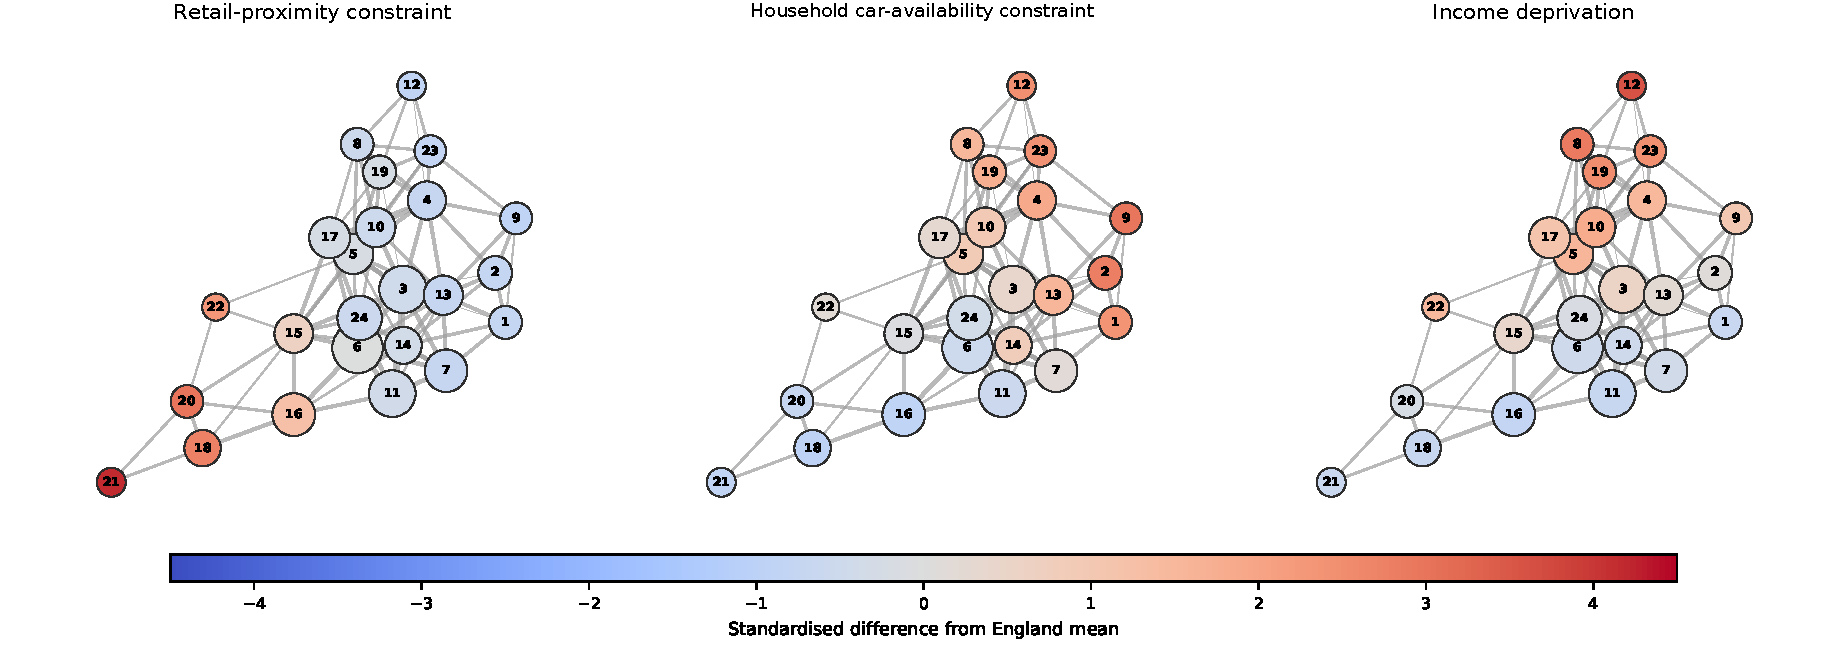
\includegraphics[width=\textwidth]{figures/figure1_canonical_bm_three_axes.pdf}
\caption{Ball Mapper representation of the three measured food-access barriers. Node positions, edges and memberships are fixed across panels. Node size reflects the number of LSOAs in each BM ball, while colour shows the ball-level standardised difference from the England mean for retail-proximity constraint, household car-availability constraint or income deprivation.}
\label{fig:canonicalbm}
\end{figure}

Barrier composition varies across the BM structure rather than forming a simple progression from low to high overall constraint. Classifying each ball-level dimension as low, near the England mean, high or very high produces 17 distinct combinations across the 24 balls (Figure~\ref{fig:axisheat}). The overall level of constraint and the composition of that constraint therefore capture different information.

\begin{figure}[htbp]
\centering
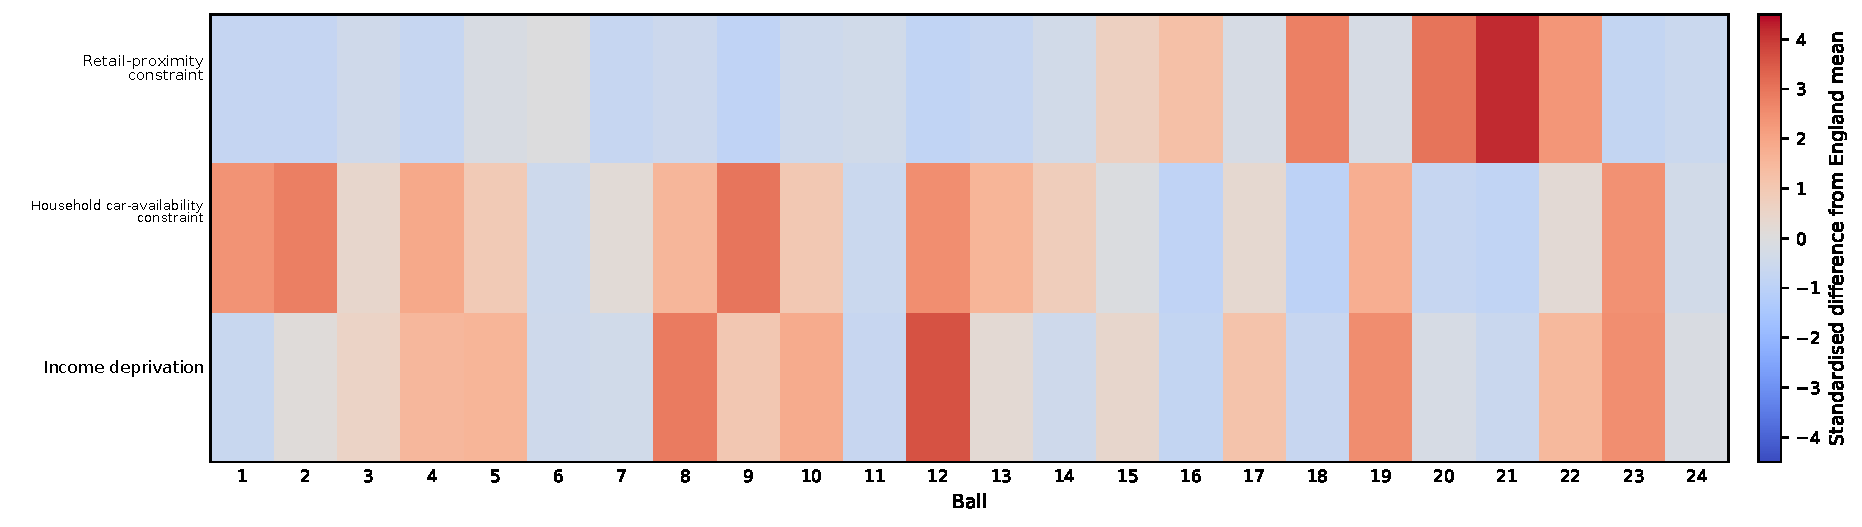
\includegraphics[width=\textwidth]{figures/figure2_topology_axis_heatmap.pdf}
\caption{Retail-proximity constraint, household car-availability constraint and income deprivation across the 24 BM balls. Cells report ball-level standardised differences from the England mean.}
\label{fig:axisheat}
\end{figure}

The illustrative three-group $k$-means benchmark captures some broad alignment but removes multiple membership by assigning every LSOA to one group. Six of the 24 BM balls have fewer than 80\% of their members assigned to the same $k$-means group. Because three groups are not treated as an optimal classification, this comparison serves only to illustrate what an exclusive assignment can compress; no central conclusion depends on it.

Contextual measures provide additional interpretation. Department for Transport shopping-connectivity scores are comparatively high in several balls with greater household car-availability constraint and comparatively low in several balls with greater retail-proximity constraint, while included-retailer counts follow a different pattern (Figure~\ref{fig:context}). The connectivity scores do not measure observed household shopping behaviour, and none of these contextual measures determines BM membership.

\begin{figure}[htbp]
\centering
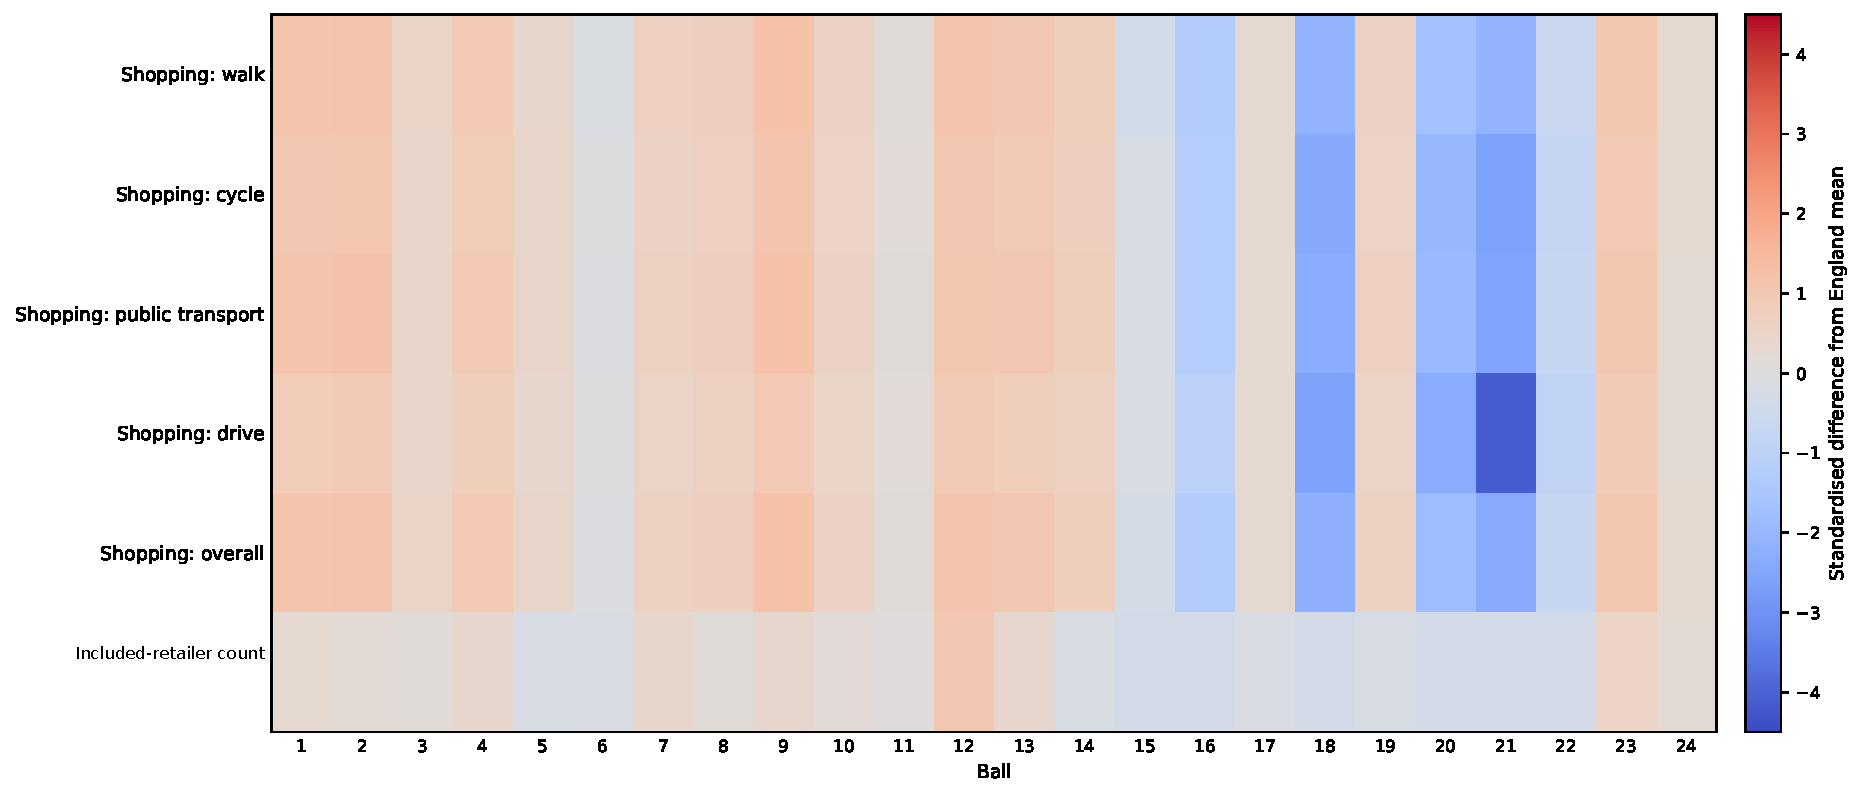
\includegraphics[width=\textwidth]{figures/figure3_context_readout_heatmap.pdf}
\caption{Selected contextual measures across the 24 BM balls. Cells report ball-level standardised differences from the England mean. Contextual measures are added after BM construction and do not determine ball membership.}
\label{fig:context}
\end{figure}
\FloatBarrier

\subsection{Similar barrier profiles recur across distant places}
Similar combinations of measured barriers are often found in places that are far apart, even though each barrier is itself geographically patterned. Moran's $I$ is 0.720 for retail-proximity constraint, 0.781 for household car-availability constraint and 0.577 for income deprivation. Yet at $k=25$, the median geographic separation among an LSOA's closest barrier-profile neighbours is 160.4 km, and 70.5\% of those neighbour relationships span more than 100 km.

Geographic proximity therefore provides only a partial guide to barrier-profile similarity. At $k=25$, 89.4\% of LSOAs share none of their 25 geographic neighbours with their 25 nearest barrier-profile neighbours. Complete separation would be even more common under independent neighbour sets, for which 98.2\% zero overlap is expected, so geography contains some information about profile similarity. Even so, it does not recover most profile neighbours. Figure~\ref{fig:spatialclosure} shows the same pattern across neighbourhood sizes from $k=5$ to $k=100$.

\begin{figure}[htbp]
\centering
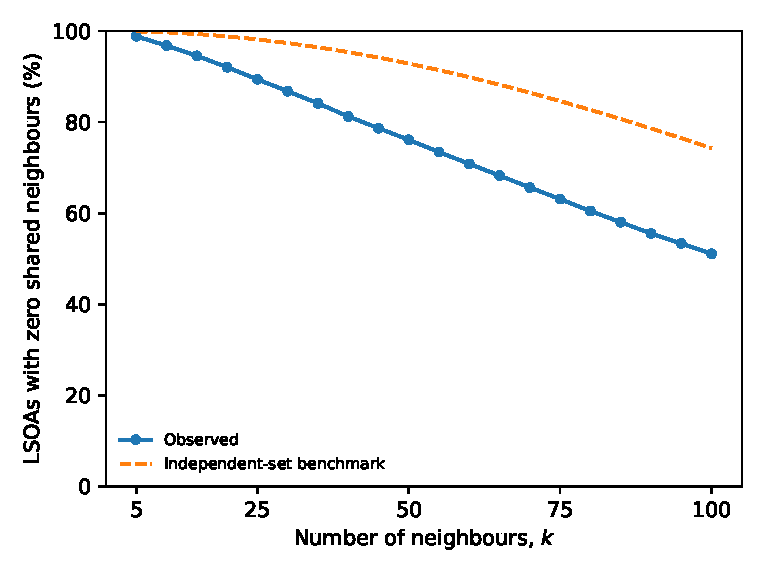
\includegraphics[width=0.68\textwidth]{figures/figure4a_zero_overlap_share.pdf}
\caption{Geographic proximity and similarity in measured food-access barriers. The figure compares the observed share of LSOAs with no common areas in geographic and barrier-profile neighbour sets with the exact independent-set expectation for $k=5,10,\ldots,100$. Observed overlap is greater than chance but remains incomplete.}
\label{fig:spatialclosure}
\end{figure}

Different barrier combinations can also occur close together. Balls 7 and 16 differ substantially across the three measured dimensions, yet their centroids are only 6.5 km apart. Their closest non-shared LSOAs are 0.37 km apart, and 2,766 immediately adjacent LSOA pairs lie across the two balls. All 24 BM balls occupy more than one contiguous geographic component. Geography matters, but geographic proximity does not reproduce the combined pattern of retail proximity, household car availability and income deprivation.

\subsection{The central finding persists across analytical choices}
The distinction between overall level and barrier composition does not depend on one BM construction or on equal weighting. Across 5,000 alternative BM constructions, every construction retains at least one BM-ball pair with a similar overall score and a clearly different barrier profile. The median share of qualifying BM-ball comparisons is 15.8\%, compared with 13.8\% in the main representation. The same substantive pattern persists when the comparison thresholds and the weights on the three barriers are changed. Supplementary Tables~S2--S5 report the full sensitivity distributions. These checks support the central result without implying that radius 1.50, the equal-weight score or the selected thresholds are uniquely preferred.

\section{Discussion}
\subsection{Overall constraint and barrier composition provide different policy information}
Our results show why the overall level of food-access constraint and its barrier composition should be treated as different pieces of policy information. Two local profiles represented by BM can appear equally constrained on a composite measure while reflecting different underlying problems. Balls 13 and 18 make that distinction concrete: almost identical overall scores arise from sharply different combinations of retail-proximity constraint, household car-availability constraint and income deprivation. An overall score describes how much measured constraint is present; barrier composition describes what that constraint consists of. Food-access research already recognises that retail provision, mobility and economic resources are not interchangeable \citep{Shaw2006,Titis2022,Beydoun2026}; the present analysis shows that the distinction is frequent enough to alter place comparison in English small-area data.

The measured barriers point to different domains for further policy assessment, but they do not prescribe interventions. Retail proximity concerns the location of included retail opportunities; household car availability describes private-vehicle resources rather than public-transport accessibility; income deprivation captures area-level income resources. A cross-sectional profile can therefore identify which measured constraints coexist without estimating whether a retail, mobility or income intervention would be effective. Place-based assessment should not infer a common barrier composition from a common overall score. The finding remains when we vary BM construction, comparison thresholds and the weights assigned to the three barriers, reducing the risk that it reflects one arbitrary analytical choice.

\subsection{Overlap and geography add information to a single score}
Ball Mapper adds a second piece of descriptive information by retaining local overlap. Most LSOAs lie within more than one BM ball, meaning that their measured profiles are similar to more than one local pattern. An exclusive classification removes that overlap by construction. The limited $k$-means comparison illustrates the difference without establishing that BM is universally preferable or that meaningful exclusive classifications cannot exist.

Geography adds context but does not provide an equivalent substitute for barrier composition. Each input dimension is spatially patterned, and geographic neighbours overlap with barrier-profile neighbours more than independent random sets would. Even so, most profile neighbours are not recovered by proximity, similar barrier profiles often occur over long distances, and contrasting profiles can occur close together. Place-based assessment should therefore use geography alongside rather than instead of the joint barrier profile. Distant profile neighbours are descriptive comparators, not causal counterfactuals.

\subsection{Relation to the food-access literature and wider policy relevance}
The findings extend rather than overturn the food-desert literature. Early UK studies established the importance of physical retail access while recognising interactions with deprivation and mobility \citep{Wrigley2002,Whelan2002,Wrigley2003}. Later work demonstrated heterogeneous intervention responses \citep{GillRudkin2014,FreireRudkin2019}, broadened access to everyday mobility and online provision \citep{Shannon2016,Newing2022,Janatabadi2024}, and developed multidimensional indices and predictive approaches \citep{Amin2021,Beydoun2026}. Our narrower contribution is to show what can be lost after multidimensionality has been recognised: a common overall level need not imply a common barrier composition.

Ball Mapper serves an instrumental role in making that distinction visible because it retains the original barrier dimensions and permits overlapping local profiles. Recent food-policy research has likewise adopted newer analytical methods when they answer a substantive representation or prediction problem rather than simply adding methodological novelty \citep{Hossain2019,Amin2021,Sartori2015}. The policy value here lies in the distinction between overall level and underlying composition, not in BM as an end in itself.

Evidence comes from England and does not establish that the same barrier profiles occur elsewhere. International relevance lies instead in the representation problem. Food-access studies in different settings combine retail opportunity, mobility resources and economic resources in different ways, and multidimensional indices increasingly summarise those conditions for policy analysis \citep{Amin2021,Cuffey2023,Pettigrew2024}. Wherever a composite score informs place-based prioritisation, retaining the underlying composition can prevent similar totals from being mistaken for similar problems. Other settings require their own measures and empirical profiles.

\subsection{Limitations}
The analysis describes area-level conditions rather than household food-shopping behaviour and does not estimate causal effects. Our deliberately parsimonious representation uses straight-line distance to the nearest included retailer, the percentage of households with no car or van, and the Income Deprivation Domain. The retailer measure covers GEOLYTIX bands B--D and excludes band A outlets below 280~m$^2$, so areas served mainly by small convenience stores may appear more retail-constrained than under a measure of all food outlets. Product-level healthfulness, food prices, food quality, cultural appropriateness, informal food sources, online behaviour, public-transport provision and individual mobility remain outside the representation. The three inputs also come from different source vintages (2021, 2023 and 2025), so they describe contemporary spatial co-occurrence on common geography rather than simultaneous conditions or change through time \citep{Dong2025,Titis2022}.

Methodological choices also define the representation. Radius 1.50 is a researcher-selected specification supported by topology diagnostics and nearby-radius sensitivity rather than an estimated optimum. Sensitivity analysis shows that the central finding persists across 5,000 nearby-radius and landmark-order constructions, alternative comparison thresholds and alternative weights, but it does not establish a unique correct BM representation. Qualifying ball pairs are descriptive comparisons rather than independent observations because BM balls overlap and individual balls enter several pair comparisons. Geographic-neighbour results likewise depend on the chosen area representation and provide descriptive rather than causal comparisons.

\section{Conclusion}
Local food-access profiles can have similar overall levels of measured constraint while reflecting different underlying barriers. Across English small areas, retail proximity, household car availability and income deprivation combine in ways that are not captured fully by a single summary score, and similar barrier profiles are not simply reproduced by geographic proximity. Ball Mapper helps retain that composition and its local overlap while keeping the original barriers available for interpretation. The central finding persists across the analytical choices examined, but its importance is substantive rather than methodological.

For policy, a composite score can still be useful for ranking or prioritising places by overall level. The score should not, however, be treated as a diagnosis of why access is constrained. Keeping retail proximity, household car availability and income deprivation visible allows a similar overall score to be interpreted in light of the barriers underlying it before further assessment. The same principle applies wherever multidimensional food-access measures inform place-based policy: overall level and barrier composition answer different questions, while intervention effectiveness requires separate causal evidence.

\section*{Data and code availability}
Source data comprise publicly available Office for National Statistics, Ministry of Housing, Communities and Local Government, Department for Transport and GeoDS data together with GEOLYTIX Retail Points Q1 2023. Source data remain subject to their respective provider licences and are not redistributed where licensing prevents this. Analysis code, source-reconstruction instructions, provenance records and non-restricted derived outputs are provided through the project repository at \url{https://github.com/srudkin12/Healthy-Food-Accessibility}. Restricted or provider-controlled source data remain available from their original providers under the relevant licences.

\section*{Declaration of generative AI and AI-assisted technologies in the writing process}
During preparation of this manuscript, Simon Rudkin used OpenAI ChatGPT for literature organisation, manuscript structuring and language editing. ChatGPT also assisted with code drafting and debugging during development of the computational workflow, as described in the Methods. All AI-assisted text and code were reviewed by the authors, empirical analyses were executed locally, and all authors take full responsibility for the submitted work.

\begin{thebibliography}{99}
\bibitem[Alexiou and Singleton(2018)]{AlexiouSingleton2018} Alexiou, A. and Singleton, A. (2018). The 2018 Internet User Classification. Geographic Data Service (GeoDS).
\bibitem[Amin et~al.(2021)Amin, Badruddoza and McCluskey]{Amin2021} Amin, M.D., Badruddoza, S. and McCluskey, J.J. (2021). Predicting access to healthful food retailers with machine learning. \emph{Food Policy}, 99, 101985.
\bibitem[Beydoun et~al.(2026)Beydoun et~al.]{Beydoun2026} Beydoun, M.A., Georgescu, M.F., Banerjee, S., Beydoun, H.A., Noren Hooten, N., Khubchandani, J., Maldonado, A.I., Tsai, J., Weiss, J., Evans, M.K. and Zonderman, A.B. (2026). Mapping food access: how neighborhood deprivation shapes healthy food availability in the United Kingdom. \emph{BMC Public Health}, 26, 1048.
\bibitem[Cuffey et~al.(2023)Cuffey et~al.]{Cuffey2023} Cuffey, J., Li, W., Yu, Y. and Miao, R. (2023). Retail food environment and household food waste: An empirical study. \emph{Food Policy}, 117, 102457.
\bibitem[Department for Transport(2025)]{DfT2025} Department for Transport (2025). Transport connectivity metric. Department for Transport, London.
\bibitem[Dłotko(2019)]{Dlotko2019} Dłotko, P. (2019). Ball mapper: a shape summary for topological data analysis. arXiv:1901.07410.
\bibitem[Dłotko et~al.(2024)Dłotko, Qiu and Rudkin]{DlotkoQiuRudkin2024} Dłotko, P., Qiu, W. and Rudkin, S.T. (2024). Financial ratios and stock returns reappraised through a topological data analysis lens. \emph{The European Journal of Finance}, 30(1), 53--77.
\bibitem[Dong et~al.(2025)Dong et~al.]{Dong2025} Dong, X., Byrne, A.T., Rhone, A. and Ver Ploeg, M. (2025). Review: untangling the complex economics of the local food retail environment. \emph{Food Policy}, 137, 102953.
\bibitem[Freire and Rudkin(2019)]{FreireRudkin2019} Freire, T. and Rudkin, S. (2019). Healthy food diversity and supermarket interventions: Evidence from the Seacroft Intervention Study. \emph{Food Policy}, 83, 125--138.
\bibitem[GEOLYTIX(2023)]{Geolytix2023} GEOLYTIX (2023). Retail Points Q1 2023. GEOLYTIX, London.
\bibitem[Gill and Rudkin(2014)]{GillRudkin2014} Gill, L. and Rudkin, S. (2014). Deconstructing supermarket intervention effects on fruit and vegetable consumption in areas of limited retail access: evidence from the Seacroft Study. \emph{Environment and Planning A}, 46, 649--665.
\bibitem[Hossain et~al.(2019)Hossain, Mullally and Asadullah]{Hossain2019} Hossain, M., Mullally, C. and Asadullah, M.N. (2019). Alternatives to calorie-based indicators of food security: An application of machine learning methods. \emph{Food Policy}, 84, 77--91.
\bibitem[Janatabadi et~al.(2024)Janatabadi, Newing and Ermagun]{Janatabadi2024} Janatabadi, F., Newing, A. and Ermagun, A. (2024). Social and spatial inequalities of contemporary food deserts: A compound of store and online access to food in the United Kingdom. \emph{Applied Geography}, 163, 103184.
\bibitem[Jenneson et~al.(2025)Jenneson et~al.]{Jenneson2025} Jenneson, V.L., Pontin, F., Ennis, E., Fildes, A., Johnstone, A.M. and Morris, M.A., on behalf of the DIO Food team (2025). Protocol for a quasi-experimental analysis: using retail sales data to evaluate impacts of the high fat, sugar and salt (HFSS) product placement restrictions legislation in England. \emph{BMJ Public Health}, 3(2), e002065.
\bibitem[Ministry of Housing, Communities and Local Government(2025)]{MHCLG2025} Ministry of Housing, Communities and Local Government (2025). English indices of deprivation 2025. Ministry of Housing, Communities and Local Government, London.
\bibitem[Newing et~al.(2022)Newing et~al.]{Newing2022} Newing, A., Hood, N., Videira, F. and Lewis, J. (2022). `Sorry we do not deliver to your area': geographical inequalities in online groceries provision. \emph{The International Review of Retail, Distribution and Consumer Research}, 32(1), 80--99.
\bibitem[Office for National Statistics(2021)]{ONS2021PWC} Office for National Statistics (2021). Lower layer Super Output Areas (December 2021) EW population weighted centroids. Office for National Statistics.
\bibitem[Office for National Statistics(2023)]{ONS2023Car} Office for National Statistics (2023). Car or van availability, Census 2021, dataset TS045, version 4. Office for National Statistics.
\bibitem[Office for National Statistics(2026)]{ONS2026RUC} Office for National Statistics (2026). 2021 Rural Urban Classification. Office for National Statistics.
\bibitem[Pettigrew et~al.(2024)Pettigrew et~al.]{Pettigrew2024} Pettigrew, S., Booth, L., Farrar, V., Brown, J., Godic, B. and Thompson, J. (2024). An emerging food policy domain: The effects of autonomous transport technologies on food access and consumption. \emph{Food Policy}, 125, 102647.
\bibitem[Pontin et~al.(2023)Pontin et~al.]{Pontin2023} Pontin, F., Baudains, P., Ennis, E. and Morris, M. (2023). Identifying drivers of food insecurity through linked data---the Priority Places for Food Index. \emph{International Journal of Population Data Science}, 8(3), 2277.
\bibitem[Rudkin et~al.(2024)Rudkin et~al.]{RudkinEtAl2024} Rudkin, S., Barros, L., Dłotko, P. and Qiu, W. (2024). An economic topology of the Brexit vote. \emph{Regional Studies}, 58(3), 601--618.
\bibitem[Sartori and Schiavo(2015)]{Sartori2015} Sartori, M. and Schiavo, S. (2015). Connected we stand: A network perspective on trade and global food security. \emph{Food Policy}, 57, 114--127.
\bibitem[Shannon(2016)]{Shannon2016} Shannon, J. (2016). Beyond the supermarket solution: Linking food deserts, neighborhood context, and everyday mobility. \emph{Annals of the American Association of Geographers}, 106(1), 186--202.
\bibitem[Shaw(2006)]{Shaw2006} Shaw, H.J. (2006). Food deserts: Towards the development of a classification. \emph{Geografiska Annaler: Series B, Human Geography}, 88(2), 231--247.
\bibitem[Titis et~al.(2022)Titis, Procter and Walasek]{Titis2022} Titis, E., Procter, R. and Walasek, L. (2022). Assessing physical access to healthy food across United Kingdom: A systematic review of measures and findings. \emph{Obesity Science \& Practice}, 8, 233--246.
\bibitem[Ver Ploeg and Wilde(2018)]{VerPloegWilde2018} Ver Ploeg, M. and Wilde, P.E. (2018). How do food retail choices vary within and between food retail environments? \emph{Food Policy}, 79, 300--308.
\bibitem[Whelan et~al.(2002)Whelan et~al.]{Whelan2002} Whelan, A., Wrigley, N., Warm, D. and Cannings, E. (2002). Life in a `food desert'. \emph{Urban Studies}, 39(11), 2083--2100.
\bibitem[Wrigley(2002)]{Wrigley2002} Wrigley, N. (2002). `Food deserts' in British cities: Policy context and research priorities. \emph{Urban Studies}, 39(11), 2029--2040.
\bibitem[Wrigley et~al.(2003)Wrigley, Warm and Margetts]{Wrigley2003} Wrigley, N., Warm, D. and Margetts, B. (2003). Deprivation, diet, and food-retail access: Findings from the Leeds `food deserts' study. \emph{Environment and Planning A}, 35, 151--188.
\end{thebibliography}

\end{document}
